\documentclass[11pt]{article}
\usepackage[margin=1in]{geometry}
\usepackage{fontspec}
\usepackage{ucharclasses}
\usepackage{graphicx}
\usepackage{booktabs}
\usepackage{array}
\usepackage{tabularx}
\usepackage{longtable}
\usepackage{hyperref}
\usepackage{xcolor}

\defaultfontfeatures{Ligatures=TeX}
\setmainfont{TeX Gyre Termes}
\newfontfamily\hangulfont[ItalicFont={Noto Sans CJK KR}]{Noto Sans CJK KR}
\setTransitionsForCJK{\hangulfont}{}{}
\setlength{\emergencystretch}{3em}
\graphicspath{{figures/}{../reports/figures/}{/home/v-seungplee/boltzmann-attention/reports/figures/}}

\title{Discovery Report: Selective Refinement, QDRP, and TRIC\\Status as of 2026-04-09}
\author{Internal Research Note}
\date{2026-04-09}

\begin{document}
\maketitle

\section*{Executive Summary}

이번 라운드의 결론은 간단하다. bounded NIAH에서 살아남은 것은 attention-path \texttt{two\_pass} selective refinement뿐이다. \texttt{query\_dequant}와 \texttt{sharp\_temp}는 같은 하네스에서 실패했고, \texttt{QDRP}는 synthetic low-budget niche만 남았으며, \texttt{TRIC}은 shared linear baseline도 넘지 못했다.

다만 이 결과를 과장하면 안 된다. 현재 \texttt{exp\_query\_exploit.py}와 \texttt{exp\_cliffkv\_niah.py}는 저장된 KV cache를 실제로 압축한 실험이 아니라 FP16 cache 위 attention path만 수정하는 diagnostic harness다. 따라서 지금 정당한 문장은 ``query-time selective refinement가 retrieval failure mode를 강하게 찌른다''이지, ``새로운 storage-valid KV-cache compression method가 이긴다''가 아니다.

\section*{Verified Facts}

\begin{longtable}{@{}p{0.08\linewidth}p{0.62\linewidth}p{0.22\linewidth}@{}}
\toprule
ID & Claim & Source \\
\midrule
\endhead
F1 & Mistral 4K same-harness에서 \texttt{baseline\_2bit = 0.333}, \texttt{two\_pass\_k16 = 1.000}, \texttt{query\_dequant\_s0.25 = 0.333}, \texttt{sharp\_temp} variants $= 0.000$. & \texttt{tmp\_remote\_results/mistral\_all\_methods\_4k.json} \\
F2 & Mistral 4K two-pass sweep에서 \texttt{k=8,16,32,64}가 모두 \texttt{1.000}. & \texttt{tmp\_remote\_results/mistral\_two\_pass\_4k.json} \\
F3 & Qwen 4K two-pass sweep에서 \texttt{k=8,16,32,64}가 모두 \texttt{1.000}. & \texttt{tmp\_remote\_results/qwen\_two\_pass\_4k.json} \\
F4 & \texttt{QDRP} diagnostic에서 \texttt{budget=1} synthetic은 도움이 되지만 \texttt{budget=2} pure risk는 악화되고 hybrid도 거의 tie다. & \texttt{reports/autoresearch\_dynamic\_recursive\_log.tsv} \\
F5 & \texttt{TRIC}은 모든 logged run에서 shared linear predictor를 이기지 못했다. & \texttt{reports/autoresearch\_dynamic\_recursive\_log.tsv} \\
F6 & 2026-04-09에 \texttt{exp\_query\_exploit.py}, \texttt{exp\_cliffkv\_niah.py}, \texttt{exp\_query\_risk\_paging.py}, \texttt{exp\_tric\_recursive\_predictor.py} self-test가 통과했다. & local validation \\
F7 & 현재 \texttt{exp\_query\_exploit.py}와 \texttt{exp\_cliffkv\_niah.py}는 attention-path diagnostic limitation을 코드에 명시한다. & code inspection \\
\bottomrule
\end{longtable}

\section*{Direction Assessment}

\subsection*{Selective Refinement}

\textbf{Intent.} low-bit key approximation으로 무너진 retrieval을 decode 시점의 selective refinement로 복구할 수 있는지 본다.

\textbf{Result.} F1--F3 기준으로 bounded 4K NIAH에서는 강하게 통과한다. 하지만 grid가 너무 쉬워 이미 포화되었고, storage path가 아직 진짜 compressed cache가 아니므로 방법 claim으로 바로 올리면 안 된다.

\textbf{Verdict.} 강한 failure-mode diagnostic으로 유지한다. paper-worthy 방향으로 살리려면 storage-valid selective side buffer 구현이 먼저다.

\subsection*{QDRP}

\textbf{Intent.} raw score가 아니라 score margin과 quantization uncertainty를 같이 써서 flip risk가 큰 page만 refinement한다.

\textbf{Result.} synthetic low-budget에서는 win이 있지만 real trace proxy는 raw score보다 약하다. 예산이 2 page로 늘어나면 pure risk는 오히려 현재 winner page를 놓친다.

\textbf{Verdict.} \texttt{budget=1} niche diagnostic 외에는 당분간 중단한다.

\subsection*{TRIC}

\textbf{Intent.} 레이어 간 KV redundancy를 shared recursive predictor로 설명하고 innovation residual만 저장한다.

\textbf{Result.} recursive predictor는 copy-last보다만 좋고, shared linear baseline은 전혀 넘지 못한다.

\textbf{Verdict.} 현재는 중단이 맞다. 다시 열려면 실제 KV trace에서 linear baseline을 넘는 증거가 먼저 나와야 한다.

\section*{What Still Needs To Be Ruled Out}

\begin{tabularx}{\linewidth}{@{}p{0.28\linewidth}X@{}}
\toprule
Alternative explanation & Why it matters \\
\midrule
Recency artifact & \texttt{two\_pass}가 needle이 아니라 query 직전 토큰을 주로 집는다면 retrieval-specific story가 무너진다. \\
Attention sink artifact & BOS or early sink token overlap이 과하면 binary success가 우연히 뒤집힌 것일 수 있다. \\
Easy 4K cliff task & \texttt{k=8,16,32,64}가 모두 1.0이면 frontier는 아직 하나도 모른다. \\
Binary NIAH saturation & top-1 success만 보고 ranking 전체 복구라고 착각할 수 있다. \\
Budget cheating & 저장 budget, HBM budget, extra compute를 분리하지 않으면 reviewer objection을 못 막는다. \\
\bottomrule
\end{tabularx}

\section*{Figures}

\begin{figure}[h]
\centering
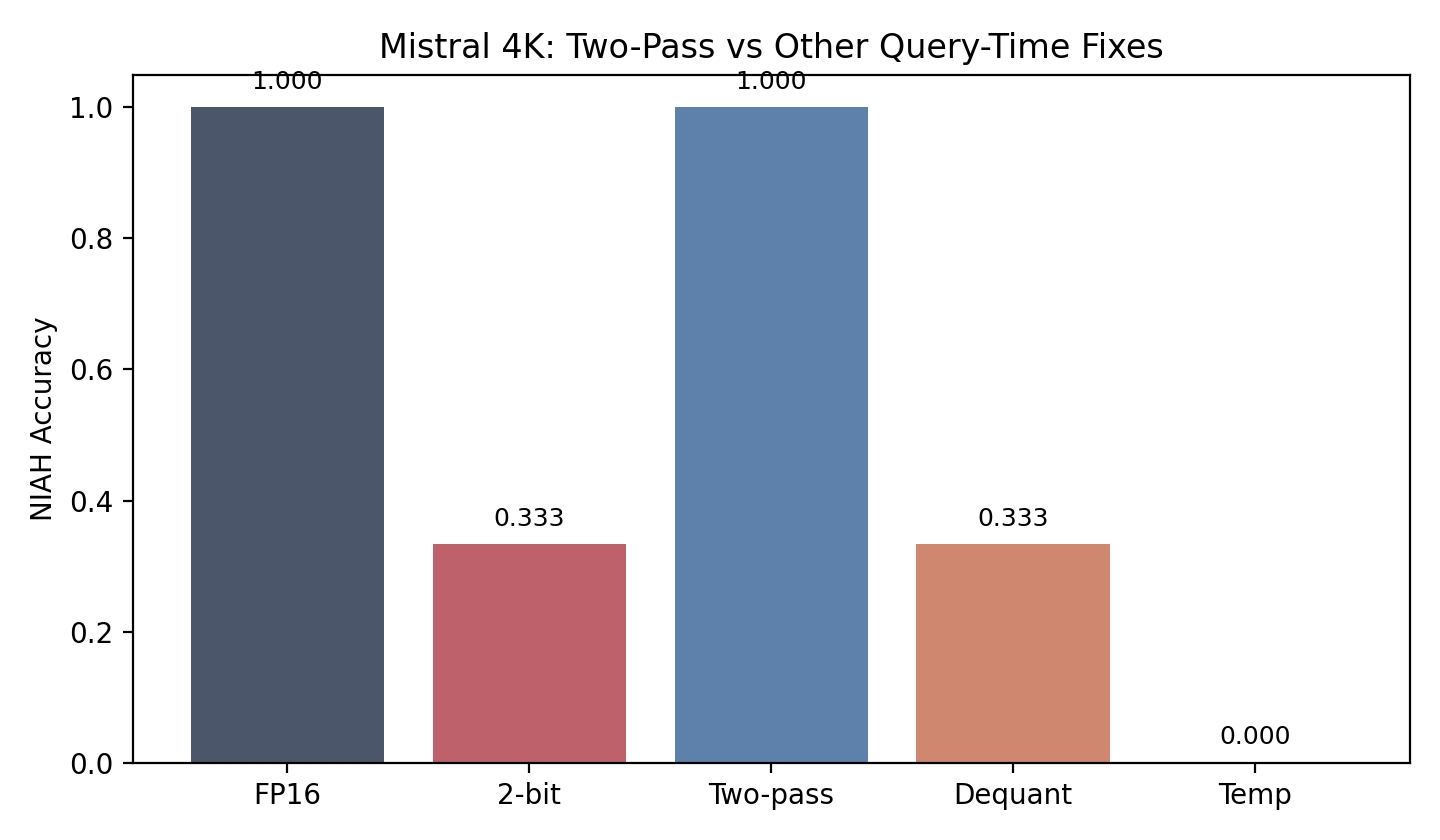
\includegraphics[width=0.8\linewidth]{selective_refine_mistral_method_compare.png}
\caption{Mistral 4K same-harness comparison. \texttt{two\_pass}만 baseline을 명확히 넘고, \texttt{query\_dequant}와 \texttt{sharp\_temp}는 실패한다.}
\end{figure}

\begin{figure}[h]
\centering
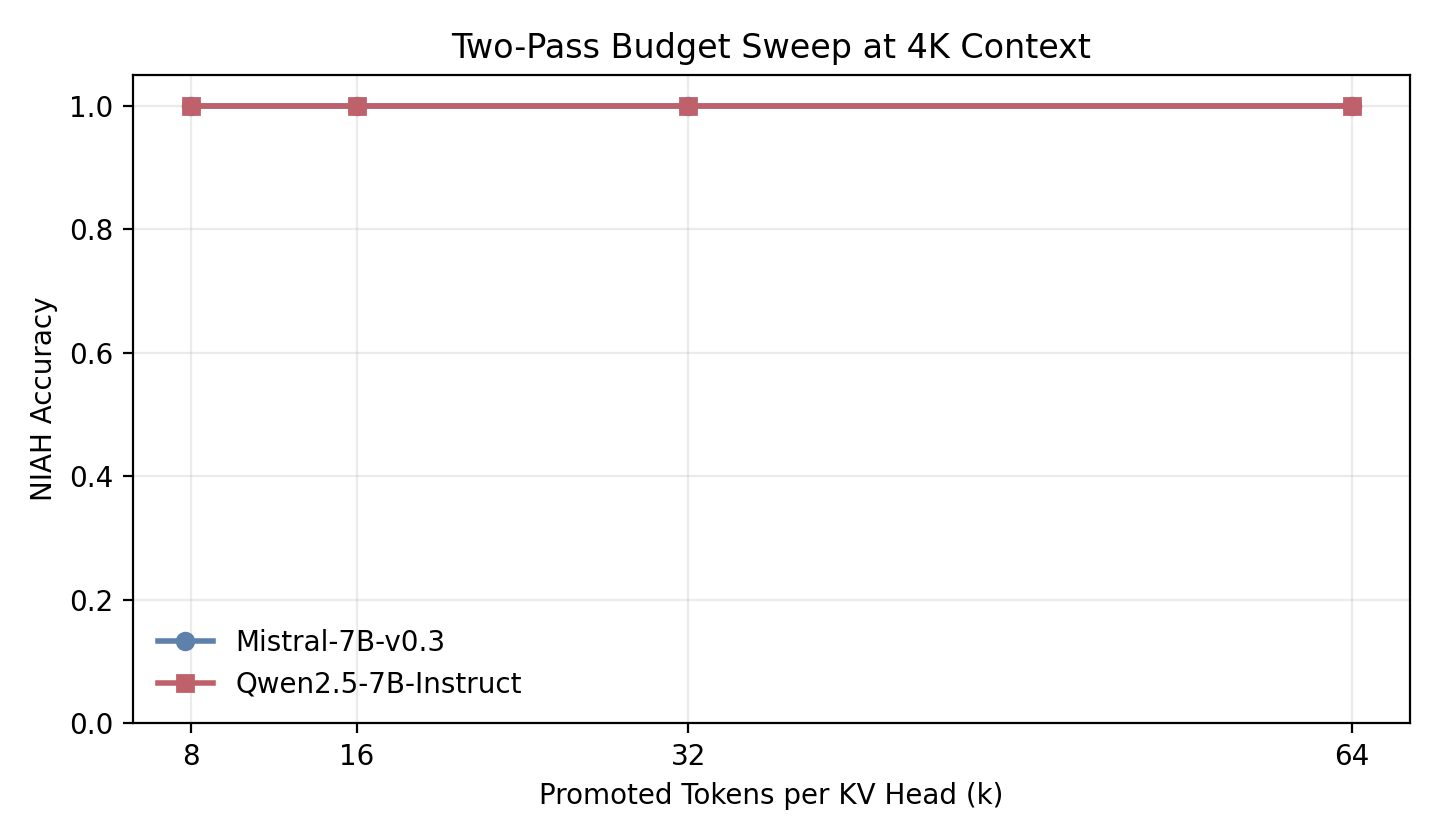
\includegraphics[width=0.8\linewidth]{selective_refine_two_pass_budget_sweep.png}
\caption{4K bounded sweep is already saturated for both models, so it demonstrates existence of the effect but not the minimum useful budget frontier.}
\end{figure}

\section*{Next Plan}

다음 실험은 네 개로 제한한다.

\begin{enumerate}
\item storage-valid selective refinement write path 구현
\item \texttt{two\_pass} vs \texttt{recent\_k}/\texttt{sink\_k}/\texttt{random\_k} control 비교
\item 8K/16K에서 \texttt{k = 1,2,4,8,16} frontier 측정
\item stored-byte matched table vs \texttt{uniform\_3bit}
\end{enumerate}

이 네 개 중 둘 이상이 실패하면 selective refinement도 논문 방법이 아니라 내부 diagnostic으로 내리는 것이 맞다.

\end{document}
